% !TeX spellcheck = pl_PL 
\chapter{Specyfikacja wewnętrzna}
\section{Struktura danych}
Reprezentację grafów w pamięci komputera można wykonać na dwa sposoby:
\begin{itemize}
	\item \textit{niskopoziomowy}: grafem jest macierz $ n\times n $ liczb całkowitych, gdzie $ n $ to liczba wierzchołków.\cite{id:AlgorytmyStruktury}
	\item \textit{wysokopoziomowy}: wierzchołki i łuki grafu są zakapsułkowane do osobnych klas.\cite{id:ZaawansowaneAlgorytmyStruktury}
\end{itemize}
W swojej pracy wybrałem drugie podejście. Poprawne zdefiniowanie klas i zależności między nimi pozwala mi w intuicyjny sposób implementować algorytmy z pseudokodu: operacje rodzaju \textit{"wykonaj daną instrukcję na wszystkich krawędziach"} można łatwo odwzorować pobierając kolekcję krawędzi i dodając im odpowiednią metodę. Nie ma potrzeby adaptować operacji na zupełnie inną strukturę.
\begin{figure}[H]
	\centering
	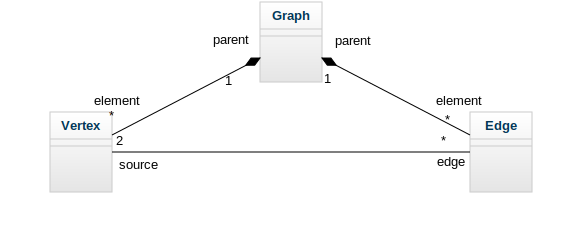
\includegraphics[width=0.6\textwidth]{./img/dane}
	\label{fig:graphStructure}
	\caption{Diagram klas struktury sieci}
\end{figure}
Zgodnie z definicją w \ref{ssec:graphDef}, graf (\emph{Graph}) składa się z dwóch zbiorów, wierzchołków (\emph{Vertex}) oraz łuków (\emph{Edge}). Graf jest kompozytem, wierzchołki i łuki stanowią jego ciało, a usunięcie obiektu grafu powoduje usunięcie jego wszystkich podrzędnych elementów. Wierzchołek jest niezależnym elementem, z kolei łuk posiada referencje do dwóch obiektów klasy wierzchołka - łuk nie może istnieć bez pary wierzchołków, które go tworzą, a usunięcie wierzchołka powoduje usunięcie wszystkich łuków wychodzących i wchodzących do niego.
\section{Konfiguracja wyglądu sieci}
Każdy obiekt sieci przepływowej posiada swoją konfigurację, w której znajdują się informacje dotyczące rysowania sieci. Każda sieć musi posiadać istniejącą konfigurację, jest to wymuszone poprzez jej konstruktor.
\begin{minted}
[
frame=lines,
framesep=2mm,
]{cpp}
explicit FlowNetwork(GraphConfig * config);
\end{minted}
Wierzchołki i łuki sieci przepływowej podczas wydarzenia rysowania pobierają swoje ustawienia z rodzica. Klasa \lstinline|GraphConfig| zawiera w sobie pięć składowych: nazwę sieci oraz cztery konteksty - sposób rysowania zwykłego elementu oraz zaznaczonego.\vfill
\cppcode{./listings/GraphConfig.cpp}
Informacje o sposobie rysowania wierzchołka są zawarte w klasie \mintinline{cpp}{VertexContext}, a łuki w klasie \mintinline{cpp}{EdgeContext}. Idea oparta jest o wzorzec \textbf{\textit{Pyłku}}. Każdy obiekt wierzchołka i łuku posiada swój niezmienny stan wewnętrzny, jak identyfikator oraz pozycję, a także stan zewnętrzny, jakim jest kolor i kształt\cite{id:WzorceProjektowePylek}. Kontekst oznacza właśnie stan zewnętrzny, którymi grafy mogą się różnić. Każdy wierzchołek i łuk posiada swój wskaźnik na aktualny kontekst, a w momencie, gdy następuje kliknięcie w elementu graf i mechanizm \textit{Qt} wykrywa zmianę zaznaczenia, wskaźnik wskazuje na przeciwny kontekst.
\cppcode{./listings/itemChange.cpp}
\section{Serializacja sieci}
Zapis oraz odczyt plików z grafami odbywa się w klasie \lstinline|GraphSerializer|. Posiada ona dwie publiczne metody:
\begin{itemize}
	\item \mintinline{cpp}{void serialize(GraphImage const & graph, std::string const & fileName);}\\
	Metoda \textit{serialize} przyjmuje jako parametr referencję do graficznej reprezentacji grafu, który ma zapisać oraz nazwę pliku wyjściowego wraz ze ścieżką.
	\item \mintinline{cpp}{GraphImage * deserialize(std::string const & filePath);}\\
	Metoda \textit{deserialize} przyjmuje jako parametr ścieżkę do pliku, który ma odczytać. Zwraca wskaźnik do graficznej reprezentacji grafu odczytanego z pliku.
\end{itemize}
Sieci przepływowe są zapisywane do formatu XML. W celu obsługi tego języka, klasa \lstinline|GraphSerializer| korzysta z darmowej biblioteki do parsowania plików XML, \emph{RapidXML}, autorstwa Marcina Kalicińskiego\footnote{Strona domowa \textit{RapidXML}: \url{http://rapidxml.sourceforge.net/}}
\subsection{Format pliku XML}
Plik zaczyna się od korzenia o nazwie \lstinline[language=XML]|<Graph>|. Format pliku można podzielić na dwie części, konfiguracyjną (gałąź \lstinline[language=XML]|<Config>|) i modelową (gałąź \lstinline[language=XML]|<Model>|). W pierwszej znajdują się globalne ustawienia wyglądu, jak rozmiary i kolory wierzchołków i łuków. Druga część zawiera model sieci przepływowej - zarówno pozycje i numery wierzchołków, jak i ich połączenia poprzez krawędzie, ich kierunek, przepustowość, przepływ oraz położenie napisu z informacją. Przykładowa sieć przepływowa oraz jej serializacja do pliku znajduje się w dodatku \ref{add:A}.


\section{Algorytmy}
Wszystkie trzy algorytmy wykonane w tej pracy zostały zakapsułkowane do osobnych klas. Ich klasą bazową bazową jest \lstinline|FlowNetworkAlgorithm|, która definiuje interfejs algorytmów oraz zawiera wspólną dla wszystkich funkcjonalność.
\subsection{Tworzenie sieci residualnej}
Algorytm służący do wygenerowania sieci residualnej jest niezmienny dla wszystkich klas i jest zawarty w metodzie klasy \lstinline|FlowNetworkAlgorithm|.
\begin{minted}[
frame=lines,
framesep=2mm,
]{cpp}
int makeResidualNetwork(FlowNetwork * network, FlowNetwork *& outResidaulNetwork)
\end{minted}
Funkcja przyjmuje dwa parametry:
\begin{itemize}
	\item \emph{network} jest siecią przepływową na podstawie której jest utworzona sieć przepływowa
	\item \emph{outResidaulNetwork} jest referencją na wskaźnik do obiektu sieci, która będzie siecią residualną. W pierwszym kroku jest to głęboka kopia sieci przepływowej.
\end{itemize}
Wartością zwracaną jest najkrótsza odległość między źródłem, a ujściem, jeżeli tworzona sieć jest \textit{warstwową siecią residualną}. Jeżeli nie jest, funkcja zwraca zero. W pierwszym kroku, algorytm usuwa wszystkie łuki z wyjściowej sieci residualnej zostawiając same wierzchołki. Następnie przechodzi przez wszystkie łuki sieci przepływowej i wykonuje poniższy algorytm.
\begin{algorithm}
	\caption{Tworzenie nowego łuku w sieci residualnej}\label{siecResidualnaPseudo}
	\begin{algorithmic}
		\Procedure{Utwórz nowy łuk}{Łuk w sieci przepływowej}
			\State{Oblicz przepustowość residualną}
			\If{Istnieje łuk sąsiedni oraz łuk sąsiedni nie został odwiedzony}
				\State{Oblicz przepływy między wierzchołkami zgodnie z zachowaniem przepływu netto w \ref{ssec:netto}}
				\State Dodaj łuk oraz łuk sąsiedni do odwiedzonych
			\EndIf
			\If{Przepływ w łuku $\ne0$}
				\State{Utwórz nowy łuk w sieci residualnej w tym samym kierunku o przepustowości równej przepływowi}
			\EndIf
			\If{Przepustowość residualna $\ne0$}
				\State{Utwórz nowy łuk w sieci residualnej w przeciwnym kierunku o przepustowości równej przepustowości residualnej}
			\EndIf
		\EndProcedure
	\end{algorithmic}
\end{algorithm}
Utworzenie tablicy odwiedzonych łuków ma zapewnić, że w sieci residualnej nie zostaną utworzone nadmiarowe łuki gdy pętla dojdzie do sąsiada. Pełny kod algorytmu znajduje się dodatku \ref{add:B}.
\subsection{Szukanie ścieżki powiększającej}
%Funkcja przeszukuje przekazaną siec przepływową i szuka w niej możliwej ścieżki powiększającej. Jeżeli ścieżka została znaleziona zwraca uporządkowaną listę wskaźników na łuki, czyli drogę, która jest powiększającą ścieżką, a do referencji \lstinline|capacity| przekazuje wartość o jaką należy zwiększyć przepływ oraz zwiększa maksymalny przepływ o tę wartość. Jeżeli ścieżka nie istnieje, zwracana lista jest pusta, a przypływ pozostaje ten sam. Ponadto, w ramach optymalizacji, funkcja sprawdza czy ścieżki powiększającej w ogóle warto szukać: jeżeli w sieci residualnej nie istnieje łuk prowadzącej ze źródła lub do ujścia, to aktualny przepływ na pewno jest maksymalny.
\subsection{Zwiększenie przepływu w sieci}
\subsection{Warunki stopu}
\subsection{Algorytm Forda-Fulkersona}
\subsection{Algorytm Dinica}
\subsection{Algorytm MKM}
